%Arquivo contendo o capítulo Estado da Arte
\chapter{Estado da Arte} \label{cap:estadoarte}
Nesta seção serão descritos alguns trabalhos relacionados com a temática e conceitos do Pedal-to-Play. Eles serão divididos em dois grupos: aplicativos comerciais e trabalhos científicos.

\section{Aplicativos comerciais}
Entre os aplicativos comerciais mais populares atualmente na categoria de Saúde e \textit{Fitness}, com a atividade de ciclismo como um dos focos, estão o Strava e o Rustatic. Ambos utilizam funções do GPS para traçar rotas, guardar trajetos do usuário e calcular valores de velocidade, altitude e distância percorrida, com a intenção de gerar relatórios sobre o desempenho do usuário em corridas ou pedaladas. \par 

O Strava, em particular, utiliza alguns conceitos de gamificação, tais como: sistema de desafios e recompensas (baseadas em prêmios, \textit{raking} e \textit{badges}); criação de metas e socialização entre usuários. \par 

Estes aplicativos também possibilitam integração com redes sociais e compartilhamento de dados entre os usuário. Assim como interfaceamento com outros dispositivos eletrônicos para monitoramento de atividades, tal como o Garmin\footnote{\url{http://www.garmin.com/}} (figura \ref{fig:garmin}). \par 

\begin{figure}[h]
    \caption{Computador compacto para bicicleta com GPS da Garmin.}
    \centerline{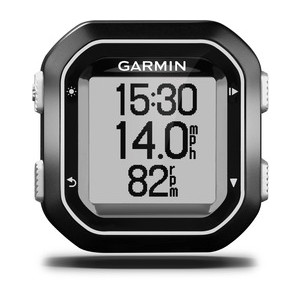
\includegraphics[width=11em]{figuras/cf-lg.jpg}}
    \label{fig:garmin}
\end{figure}
\centerline{Fonte: Página oficial do produto na \textit{Web}\footnote{Disponível em:  <\url{https://buy.garmin.com/pt-BR/BR/cIntoSports-cCycling-p1.html}>. Acesso  em jun. 2015.}}

\section{Trabalhos científicos}
Entre os trabalhos científicos pesquisados estão as obras de Cesani e Dranka \citeyearpar{cesani2013} e Rosero \citeyearpar{gaidos2012}, ambos propuseram sistemas em \textit{software} para auxiliar ciclistas em suas atividades. \par

Cesani e Dranka propuseram diretrizes para o desenvolvimento de uma aplicação \textit{mobile} com a intenção de auxiliar os ciclistas de Curitiba em seus trajetos. Para isso, eles estudaram o sistema de navegação GPS; as ciclovias e vias alternativas de Curitiba; o perfil do ciclista desta cidade; documentos sobre a infraestrutura urbana cicloviária e produtos relacionados usados pelos ciclistas de Curitiba. Como resultados, os autores definiram a fundamentação teórica da pesquisa e uma base para o desenvolvimento da interface homem-computador para um futuro protótipo funcional. \par

Rosero, em sua dissertação de mestrado, desenvolveu um protótipo para um sistema de treinamento e monitoramento para ciclistas (figura \ref{fig:rosero}). Envolvendo a implementação de uma aplicação para plataforma Android e módulos de \textit{hardware} (tais como um módulo Bluetooth\footnote{Bluetooth é uma tecnologia de comunicação sem fio, baseada em ondas de rádio frequência de curto alcance. Possibilita comunicação eficiente e eficaz entre diferentes dispositivos eletrônicos \cite{gaidos2012}.}, sensores de frequência cardíaca, de percentual de oxigênio e de temperatura). Este sistema fornece informações dos sinais fisiológicos do usuário, processando e disponibilizando estas na rede social Twitter\footnote{\url{https://twitter.com}}, para que um treinador possa acompanhar os resultados.

\begin{figure}[hb]
    \caption[Protótipo de \textit{hardware} desenvolvido por Rosero ligado ao capacete de um ciclista]{Protótipo de \textit{hardware} desenvolvido por Rosero ligado ao capacete de um ciclista \cite{gaidos2012}.}
    \centerline{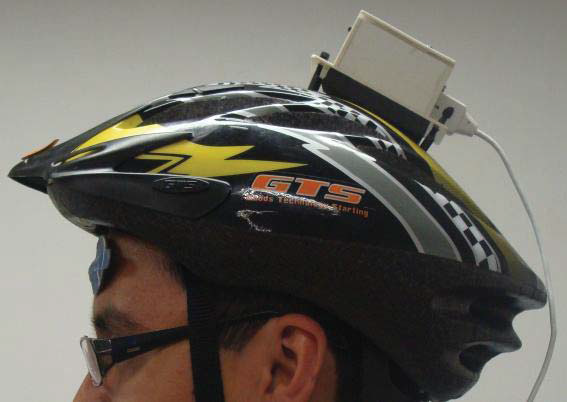
\includegraphics[width=18em]{figuras/rosero.png}}
    \label{fig:rosero}
\end{figure}